
\subsection{Кусочно гладкие поверхности}
$ S $ --- простая гладкая поверхность с кусочно гладким краем $ \delta S $. 
\paragraph{Определение.} Ориентация края $ \delta S $  поверхности $ S$ согласовывается с ориентацией поверхности $ S $, если глядя  конца вектора нормали на край он обходится против часовой стрелки.
\paragraph{Определение.} Поверхность $ S $ называется кусочно гладкой поверхностью, если ее можно представить в виде конечного объединения простых гладких поверхностей, которые пересекаются разве что только по общим краям\\
\begin{minipage}{110mm}
	\begin{center}
		$ S = \text{\tmb{m}{\cup}{k=1}} S_k,\; S_k\text{ --- простая гладкая поверхнсоть} $
	\end{center}
\textbf{Пример.} $ S = \{ \overline{r}=\overline{r}(\varphi,\psi),\; 0\leqslant\varphi \leqslant 2\pi,\; -\pi/2 \leqslant \psi \leqslant \pi/2  \} $ --- сферические координаты.\\
$ S: \; x^2+y^2+z=1 $\\
$ S_1 = \{ z=\sqrt{1-x^2-y^2},\; x^2+y^2=1/2  \};\\ S_2 = \{ z=-\sqrt{1-x^2-y^2},\;x^2+y^2=1/2 \} $\\
$ S_3 = \{ \overline{r}=\overline{r}(\varphi, \psi),\; \abs{\psi}\leqslant\pi/4,\; 0\leqslant\varphi\leqslant\pi\};\\ S_4 = \{ \overline{r}=\overline{r}(\varphi, \psi),\;\abs{\psi}\leqslant\pi/4 ,\;\pi\leqslant\varphi\leqslant2\pi \} $
\end{minipage}
~
\begin{minipage}{60mm}
	\begin{figure}[H]
		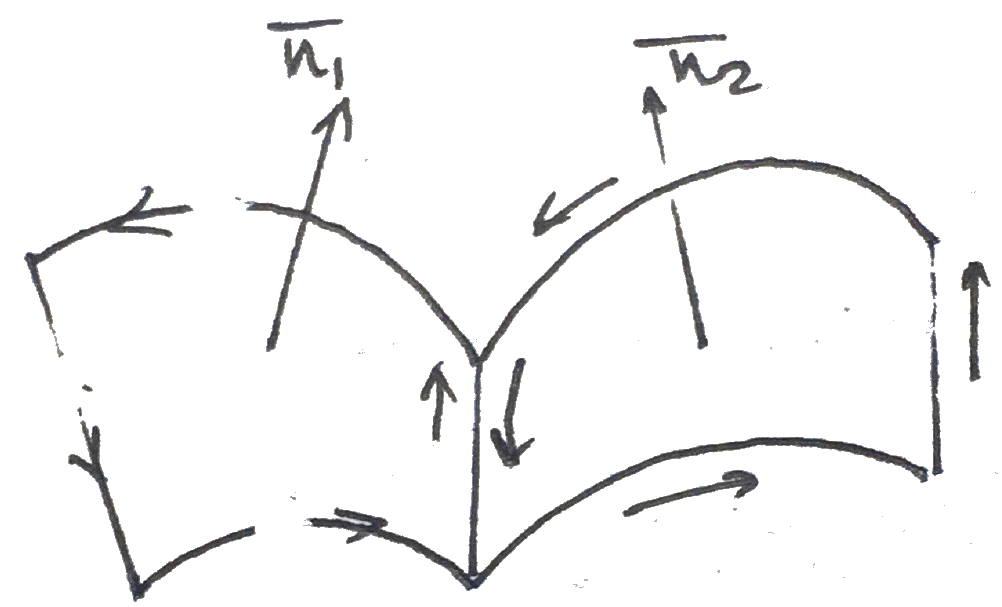
\includegraphics[width=60mm]{img3}
		\caption{$ \overline{n} = \{ \overline{n_1}, \ldots, \overline{n_m} \} $}
	\end{figure}
\end{minipage}